\chapter{Обзор литературы} \label{chapt1}

В данной главе будет проведен обзор литературы по 

\section{Метод линейной комбинации атомных орбиталей} \label{sect1_1}

\subsection{Атомная теория Бора}

У истоков современной теории химической связи стоял Н. Бор, который в 1913 году предложил теорию строения атомов для объяснения спектров атома водорода. 
Он утверждал, что в атоме H вокруг ядра вращается по круговой орбите электрон, удерживаясь на ней благодаря равновесию между центробежной силой и силой электростатического притяжения отрицательно заряженного электрона и положительно заряженного ядра.
Бор предположил, что электрон может находится лишь на строго определенных расстояниях от ядра, каждое из которых соответствовало своей орбитали.
Эта орбиталь характеризовалась так называемым главным квантовым числом $n$, которое могло принимать лишь положительные целочисленные значения.
С увеличением главного квантового числа увеличивается энергия электрона, находящегося на соответствующей орбитали. 
Т.е. электрон в невозбужденном атом водорода находится на орбитали с $n=1$, а в случае если атом начинают выводить из состояния равновесия, например облучая его внешним источником, электрон может переходить на орбитали обладающие повышенной энергией.

Однако, эта теория хорошо могла описывать только одноэлектронные системы, что вызвало необходимость усовершенствования теории Бора.
Первое усоверщенствование предложил А. Зоммерфельд, который предложил ввести дополнительный параметр характеризующий орбитали, в современной теории это орбитальное квантовое число $l$, которое может принимать целочисленные значения находящиеся в диапазоне $l \in [0;n-1]$. 
Каждому значению $l$ соответствует своя форма электронной оболочки, например $l=0$ представляет из себя сферическую орбиталь, а при $l=1$ "--- гантелеобразную. 
Для обозначения орбиталей используются определенные строчные буквы английского алфавита: $s(l=0)$, $p(l=1)$, $d(l=2)$ и~т.д.

Заполнение электронной оболочки следует согласно следующим трем принципам. 
Первый принцип заключается в том, что электроны стремятся заполнить орбитали с наименее возможной энергией. 
Следующий ряд показывает порядок заполнения первых нескольких орбиталей: $1s<2s<2p<3s<3p<4s<3d<4p...$ Согласно второму принципу (принцип Паули), одну орбиталь могут занимать только два электрона, но эти два электрона должны иметь противоположный спин. 
Третий принцип --- правило Гунда --- гласит, что электроны сначала стремятся заполнить все вырожденные орбитали по одному, имея при этом одинаковые спины, после чего полностью заполняют орбитали.

Последующее развитии этой теории заключается в разработке математического аппарата квантовой механики. 
В последствии получилось развить этот аппарат и на более сложные системы, не ограниченные одним ядром, но также на молекулы и полимерные структуры.

\subsection{Электронный гамильтониан и электронное строение атомов и молекул}

Электронное строение молекулы "--- системы электронов, находящихся в электрическом поле ядер, координаты которых известны, определяются из многоэлектронной волновой функции $\Psi_k$, зависящей от координат всех входящих в нее электронов \cite{landau1974,davidov1973,sleiter1969}. 
Собственные функции $\Psi_k$ и энергии электронных орбиталей можно найти из стационарного уравнения Шрёдингера \ref{eq:shredStat}
\begin{equation}
\label{eq:shredStat}
H\Psi_k=E_k\Psi_k,
\end{equation}
где $H$ --- полный гамильтониан системы электронов и атомных ядер;
\begin{equation}
\label{eq:fullHam}
H=T_e+V_{ee}+V_{en}.
\end{equation}

В уравнении \ref{eq:fullHam} первое слагаемое характеризует кинетическую энергию электрона, второй --- кулоновское взаимодействие между электронами, и последнее --- кулоновское взаимодействие между электронами и ядрами. 
Зависимости для каждого из составляющих представлена в уравнениях~\ref{eq:T_e}-\ref{eq:V_en}

\begin{eqnarray}
\label{eq:T_e}
T_e=-\sum_{i=1}^{N}\frac{\hbar^2}{2m}\left(\frac{\partial^2}{\partial x^2}+\frac{\partial^2}{\partial y^2}+\frac{\partial^2}{\partial z^2}+\right), \\
\label{eq:V_ee}
V_{ee}=\sum_{i<j}^{N}\frac{e^{2}}{\biggl((x_i-x_j)^2+(y_i-y_j)^2+(z_i-z_j)^2\biggr)^{0.5}}, \\
\label{eq:V_en}
V_{en}=\sum_{i=1}^{N}\sum_{j=1}^{N_n}\frac{\zeta_j e^{2}}{\biggl((x_i-X_j)^2+(y_i-Y_j)^2+(z_i-Z_j)^2\biggr)^{0.5}},
\end{eqnarray}
где $m$ и $e$"--- масса и заряд электрона, $\hbar$ "--- постоянная Планка, $\zeta_j$ "--- заряды ядер, $N$ "--- число электронов, $N_n$ "--- число ядер; $x_i$, $y_i$, $z_i$ "--- пространственные координаты электронов;$X_i$, $Y_i$, $Z_i$ "--- декартовы координаты ядер.

Волновая функция $\Psi_k$ должна быть всюду непрервывна и однозначна, также как и её первая производная. Она должна быть удовлетворять условиям \ref{eq:shredStat}, \ref{eq:invar} т.е. при интегрировании по всему пространству квадрат ее должен равняться единице, а также при перестановке двух электронов должна менять знак
\begin{eqnarray}
\label{eq:norm}
\int_{V}\Psi_kdr=1, \\
\label{eq:invar}
\Psi_k(a_1,a_2,a_3...)=-\Psi(a_2,a_1,a_3...),
\end{eqnarray}
где $V$ обозначает интегрирование по всему пространству, $a_i$ "--- совокупность трех декартовых координат электрона и спина электрона. 
Полная энергия многоатомной системы состоит из комбинации описанных выше составляющих полную электронную энергию и энергию отталкивания ядер $V_nn$:
\begin{equation}
V_nn=\sum_{i<j}^{N_n}\frac{\zeta_i\zeta_j e^{2}}{\biggl((X_i-X_j)^2+(Y_i-Y_j)^2+(Z_i-Z_j)^2\biggr)^{0.5}}.
\end{equation}

Нахождение значений энергии $E_k$, удовлетворяющих уравнению~\ref{eq:shredStat} и является основной задачей теории электронного строения атомов, молекул и кристаллов.

\subsection{Молекулярные и атомные орбитали}

Волновая функция $\Psi_k$ дает полную информацию об электронной системе, однако пользуясь только уравнением \ref{eq:shredStat} невозможно рассчитать не то, что сложную многоядерную систему, но даже систему имеющую больше одного электрона. 
Для разрешения этой проблемы используют физически обоснованные предположения о виде многоэлектронной волновой функции. 
Одно из таких приближений состоит в представлении волновой функции многоэлектронной системы в виде детерминанта, матрицы составленной из одноэлектронных волновых функций \ref{eq:T_e}-\ref{eq:V_en}:
\begin{equation}
\label{eq:LCAO}
\Psi_k=\frac{1}{\sqrt{N!}}\det 
\begin{Vmatrix}
\phi_1(a_1) & \phi_2(a_1) & \cdots & \phi_N(a_1) \\
\phi_1(a_2) & \phi_2(a_2) & \cdots & \phi_N(a_2) \\
\cdots & \cdots & \ddots & \cdots \\
\phi_1(a_N) & \phi_2(a_N) & \cdots & \phi_N(a_N) 
\end{Vmatrix},
\end{equation}
здесь $\phi_j(a_i)$ "--- волновая функция одноэлектронной системы, называемая спин-орбиталью, которая представляет из себя произведение спиновой составляющей и пространственной $\psi_j(x_i,y_i,z_i)$. 
Последняя называется орбиталью. 
В случае атомов $\psi_j$ называется атомной орбиталью, для молекул "--- молекулярной, для случая кристаллов или полимеров она имеет вид блоховских функций. 
Спиновая же составляющая может принимать лишь два значения +1/2 и -1/2.

В уравнении \ref{eq:LCAO} коэффициент $N^{-0.5}$ необходим, для обеспечения нормировки волновой функци:
\begin{eqnarray}
\label{eq:normBasis}
\int\phi^2_jdv=1,\\
\label{eq:ortogBasis}
\int\phi_j\phi_idv=0, \text{ при }j\ne i.
\end{eqnarray}

Для системы с наперед заданным пространственным положением ядер, можно найти волновые функции $\psi_j$ и собственные значения энергий $E_j$ используя вариационный метод, который говорит, что чем ближе подходим к точной волновой функцией, тем ниже значение собственной энергии. 
Вид орбитали $\psi_j$ находится из стационарного одноэлектронного уравнения Шрёдингера \ref{eq:shredOne}. 
Вид оператора гамильтона представлен в уравнении \ref{eq:hamOne}.

\begin{eqnarray}
\label{eq:shredOne}
H\psi_i=E_i\psi_i,\text{ где }i=1,2\dots\\
\label{eq:hamOne}
H=-\Delta+U(r)
\end{eqnarray}

В уравнении \ref{eq:hamOne} первое слагаемое отвечает за кинетическую энергию электрона, второе за кулоновское взаимодействие между конкретным электроном и другими электронами и ядрами.

Из-за того, что вид оператора $H$ зависит от искомых функций $\psi_i$, то для решения системы уравнений Харти-Фока \ref{eq:shredOne} используется следующий метод: их некоторых физических представлений берутся приблизительные функции $\psi_i$ и подставляются в систему, на основе которых уточняются значения оператора Хартри-Фока, затем система уравнений снова решается с уже уточненным оператором $H$. 
Происходит последовательное уточнение базисных функций, вплоть до того момента, когда с повторением итераций изменение значения энергии достигает таких величин, которые удовлетворяют погрешности. 
По этой причине этот метод также называют методом самосогласованного поля.

\subsection{Секулярное уравнение}

Благодаря вычислительным мощностям современных компьютеров, не составляет труда решить уравнения Хартри-Фока для всех основных одноядерных систем (атомов, ионов). 
Однако в случае многоатомных систем решение этих уравнений вызывает значительно большие трудности, поэтому для решения уравнений \ref{eq:shredOne} используются дальнейшие приближения. 
Обычно эти приближения заключаются в том, что молекулярные орбитали (МО) представляют в виде линейной комбинации других волновых (базисных) функций, в общем случае берущихся индивидуально каждый раз:
\begin{equation}
\label{eq:LCAOOne}
\psi_j=\sum_{i=1}^{n}a_{j,i}\chi_i, \text{ при } j=1,2 \dots, n
\end{equation}
где $a_{j,i}$ "--- коэффициенты определяющие вклад соответствующей базисной функции в собственную функцию $\psi_j$. 
Базисные функции подбираются таким образом, чтобы они были всюду непрерывны и дифференцируемы.

Исходя из вышеописанного приближения расчёт сложной многоядерной системы сводится к нахождению этих коэффициентов разложения $a_{j,i}$. 
Это можно сделать подставляя уравнения \ref{eq:shredOne} в \ref{eq:LCAOOne} и используя вариационный метод, получаем, так называемое, секулярное уравнение \ref{eq:seculMatrix}.

\begin{eqnarray}
\label{eq:seculMatrix}
\det 
\begin{Vmatrix}
<\chi_1|H|\chi_1>-E<\chi_1|\chi_1> & \cdots & <\chi_1|H|\chi_n>-E<\chi_1|\chi_n> \\
<\chi_2|H|\chi_1>-E<\chi_2|\chi_1> & \cdots & <\chi_2|H|\chi_n>-E<\chi_1|\chi_n> \\
\cdots &  \ddots & \cdots \\
<\chi_n|H|\chi_1>-E<\chi_n|\chi_1> & \cdots & <\chi_n|H|\chi_n>-E<\chi_n|\chi_n> \\
\end{Vmatrix}=0\\
\label{eq:seqEq}
\left\{\begin{matrix}
a_{j,1}(<\chi_1|H|\chi_1>-E<\chi_1|\chi_1>) + \cdots + a_{j,n}(<\chi_1|H|\chi_n>-E<\chi_1|\chi_n>)=0 \\
a_{j,1}(<\chi_2|H|\chi_1>-E<\chi_2|\chi_1>) + \cdots + a_{j,n}(<\chi_2|H|\chi_n>-E<\chi_1|\chi_n>)=0 \\
\cdots  \\
a_{j,1}(<\chi_n|H|\chi_1>-E<\chi_n|\chi_1>) + \cdots + a_{j,n}(<\chi_n|H|\chi_n>-E<\chi_n|\chi_n>)=0 \\
\end{matrix}\right.
\end{eqnarray}

Здесь $<\chi_k|H|\chi_i>$"---матричные элементе гамильтониана, а $<\chi_k|\chi_i>$"---интегралы перекрывания. 
Из \ref{eq:seqEq} можно определить все $a_{j,i}$ с точностью до множителя. 
Для нахождения точных значений необходимо нормировать полученную функцию \ref{eq:LCAOOne}.

\subsection{Атомный базис}

Если рассматривать мнгоатомную систему, то с довольно большой точностью можно утверждать, что когда электрон находится вблизи ядра одного из атомов, то волновая функция МО приближается по виду к АО, соответствующего атома. 
Отсюда зародилось предложение использовать в качестве базисных функций для МО волновые функции атомных орбиталей. 
Таким образом возник метод МО ЛКАО, когда молекулярные орбитали представляются в виде линейной комбинации атомных орбиталей. 
В применении этого метода к кристаллам появился метод сильной связи \cite{sleiter1978,sleiter1969,zaiman1974,levin1974}. 
При расчете в рамках метода обычно рассматривают в полной мере лишь  валентные электроны, в отличие от которых предполагается, что остовные лишь экранируют положительный заряд ядер, поэтому например для атома углерода с конфигурацией $1s^22s^22p^2$ осбуждают лишь $2s^22p^2$.

\section{Химическая связь в простейших молекулах}

\subsection{Орбитали двухатомных молекул}

В качестве простейшей двухатомной молекулы рассмотрим молекулу водорода H${}_2$. 
Процесс образования молекулы происходит при сближении двух атомов, и в тот момент когда расстояние между ядрами достигает приблизительно длины связи происходит притяжение между электроном одного атома и ядром другого. 
При этом атомные орбитали меняют свой вид на форму молекулярных двухцентровых орбиталей. 
Как было описано выше, при приблежении электрона к ядру одного из атомов, на его свойства большее влияние оказывает данное ядро, нежели другое, поэтому МО $\sigma$ приближается к виду АО $s_1$. По аналогии при смещении в сторону другого протона $\sigma$ изменяется к $s_2$. 
На основании этого можно предположить, что допустимым будет применение описанного выше метода МО ЛКАО:
\begin{equation}
\label{eq:LCAOH}
\psi_j=a_{j,1}s_1+a_{j,2}s_2, \text{ при } j=1,2.
\end{equation} 
Подставляя \ref{eq:LCAOH} в \ref{eq:seculMatrix} получаем следующее секулярное уравнение:
\begin{eqnarray}
\label{eq:seculMatrixH}
\det 
\begin{Vmatrix}
<s_1|H|s_1>-E<s_1|s_1> & <s_1|H|s_2>-E<s_1|s_2> \\
<s_2|H|s_1>-E<s_2|s_1> & <s_2|H|s_2>-E<s_2|s_2>
\end{Vmatrix}=0\\
\label{eq:seqEqH}
\left\{\begin{matrix}
a_{j,1}(<s_1|H|s_1>-E<s_1|s_1>) +  a_{j,2}(<s_1|H|s_2>-E<s_1|s_2>)=0 \\
a_{j,2}(<s_2|H|s_1>-E<s_2|s_1>) +  a_{j,2}(<s_2|H|s_2>-E<s_2|s_2>)=0
\end{matrix}\right.
\end{eqnarray}

В силу ортонормированности базисных функций \ref{eq:normBasis},\ref{eq:ortogBasis} $<s_1|s_1>=<s_2|s_2>=1$, $<s_1|s_2>=<s_2|s_1>=0$. 
Из-за симметрии молекулы водорода $<s_1|H|s_1>=<s_2|H|s_2>$ и $<s_1|H|s_2>=<s_2|H|s_1>$. 
Для упрощения записи воспользуемся двумя станадартными обозначениями $<s_i|H|s_i>=\alpha$ и $<s_i|H|s_k>=\beta$. 
В литературе \cite{streitviser1965} первый интеграл ($\alpha$) называют кулоновским, его величина практически не зависит от взаимного расположения атомов и характеризует исключительно вид атома, второй"---интеграл перескока или резонансный"---наоборот сильно зависит от расстояния между ядрами. 

Решая уравнения \ref{eq:LCAOH}-\ref{eq:seqEqH}, получается две возможные орбитали $\psi_b=(s_1+s_2)/sqrt(2)$ и $\psi_b=(s_1-s_2)/sqrt(2)$, что соответствует двум возможным структурам молекулы. 
Схематично образование МО в молекуле водорода H${}_2$ изображено на рис.~\ref{fig:H2}. 
Величины энергий соответствующих орбиталям равны $E_b=a-|b|$ и $E_a=a+|b|$. 
Собственные функция и энергия с индексом $b$ соответствуют случаю, когда электрон находится на связывающем состоянии, а индекс $a$ характеризует разрыхляющую орбиталь. 
Если рассматривать случай связывающего состояния, то можно можно увидеть, что плотность вероятности нахождения электрона больше между ядрами атомов, образуется молекула, в обратном случае вероятность нахождения электронов по разные стороны от ядер максимальна, что соответствует невозможности образования молекулы.

\begin{figure}
\center{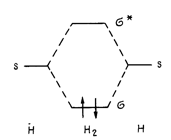
\includegraphics[scale=0.75]{H-H}}
\caption{Образование МО из АО в молекуле H${}_2$\cite{dyachkov2011}}
\label{fig:H2}
\end{figure}

В молекуле водорода, обе атомные орбитали образующие связь сферически симметричны вокруг оси соединяющей центры атомов, молекулярные орбитали, которые образуются в этом случае называются $\sigma$-орбиталями. 

Глядя на рис.~\ref{fig:H2}, удобно рассматривать и предсказывать возможность устойчивости других двухатомных систем, в образовании связи которых учавствуют $s$-орбитали. 
Для примера можно рассмотреть случай молекул и ионов H и H. 
Например можно ожидать уменьшения стабильности для иона H${}_2^+$, по аналогии и ион H${}_2^-$ должен иметь меньшую стабильность. 
Если же рассмотреть двухатомную молекулу He$_2$, то видно что как на связывающей, так и на разрыхляющей орбитали будут находиться по два спаренных электрона, и последние буду нивелировать влияние связывающего состояния на возможность образования молекулы, что доказывает невозможность ее существования.

\subsection{$\pi$-Орбитали в ненасыщенных орбиталях}

Рассматриваемые нами ранее структуры двухатомных молекул были довольно простыми по сравнению с сложными полимерными структурами молекул, такими как нанотрубки, графитовые слои, цепочки карбина. 
Также сложности по сравнению с ранее описанными структурами добавляет наличие не одной, а четырех валентных орбиталей, приходящихся на каждый атом.
Однако при изучении некоторых из соединений углерода можно разделить его орбитали на малоподвижные (глубоколежащие) орбитали $\sigma$-типа и высокоподвижные $\pi$-орбитали (рис. \ref{fig:PiSigma}).

\begin{figure}
\center{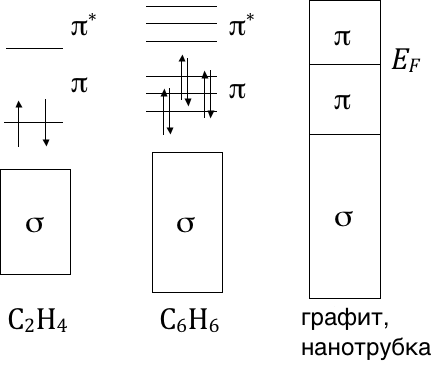
\includegraphics{PiSigmaOrbit}}
\caption{Взаимное расположение $\sigma$ 
и $\pi$ уровней в соединениях углерода 
с $\sigma$ и $\pi$ связями. $\sigma$-Уровни
 и связывающие $\pi$ состояния заполнены электронами, а разрыхляющие $\pi^{*}$ уровни вакантны. \cite{dyachkov2011}}
\label{fig:PiSigma}
\end{figure}

Низкоэнергетические возбуждение подобных системы происходят за счет переходов между занятыми и вакантными $\pi$-состояниями. 
Рассмотрим это на примере двух ненасыщенных молекул углерода: этилена и бутадиента.

Все атомы в молекуле этилена C${}_2$H${}_4$ находятся в одной плоскости XY. 
Благодаря такому расположению, МО этой системы либо симметричны, либо антисимметричны относительно этой плоскости. 
Орбитали $2s$, $2p_x$ и $2p_y$ атомов углерода и $1s$ атомов водорода образуют связи лежащие в плоскости ядер. 
Все описанные выше орбитали углерода благодаря явлению гибридизации имеют одинаковую энергию и лежат под углом $120^{\circ}$. 
Эти орбитали, симметричные относительно XY образуют $\sigma$-орбитали. 
Оставшаяся же орбиталь каждого атома углерода $2p_z$ лежит перпендикулярно плоскости ядер. 
Эта орбиталь обладает антисимметричностью, относительно XY. 
Атомные орбитали  данного типа и образуют молекулярную орбиталь, которая при отражении относительно плоскости молекулы меняет знак. 
Эти орбитали называются орбиталями $\pi$ типа. 
Подобная симметричность молекулы является причиной того, что интегралы взаимодействия $\sigma$ МО равны нулю. 
Взаимодействие $2p_z$ орбиталей вызывает образование двух $\pi$ МО:
\begin{eqnarray}
\label{eq:piBond}
\psi_b^{\pi}=(p_{z1}+p_{z2})\sqrt{2}\\
\label{eq:piAntiBond}
\psi_a^{\pi}=(p_{z1}-p_{z2})\sqrt{2}
\end{eqnarray}
По аналогии с молекулой водорода \ref{eq:LCAOH} образуется одна связывающая орбиталь \ref{eq:piBond} и одна разрыхляющая \ref{eq:piAntiBond}. 
Энергии связывающего состояния и рахрыхляющего соответственно равны $E_b=\alpha_\pi-|\beta_\pi|$ и $E_b=\alpha_\pi+|\beta_\pi|$. 
Основное состояние молекулы этилена характеризуется наличием двух электронов на связывающей $\pi$-орбитали и их отсутствием на разрыхляющей.
 Электроны на $\pi$ МО называются $\pi$-электронами.

Многие теоретические и практические работы \textbf{вставить ссылку} показали, что $\sigma$ электроны в ненасыщенных углеводородах лежат гораздо глубже по сравнению с $\pi$ электронами. 
Поэтому первые можно рассматривать, как неактивные и оказывающие влияние на систему лишь в качестве экранирующих заряд ядра. 

Теперь рассмотрим молекулу бутадиена, в которой в отличие от этилена имеется не одна изолированная двойная связь, а две сопряженные двойные связи. 
Однако как и молекула этилена бутадиен представляет собой плоской систему, в которой каждый атом углерода образует три $\sigma$-связи с соседними атомами углерода и водорода и одну $\pi$-связь. 
Все $\pi$-облака между собой пересекаются образую одну общую $\pi$-систему.

Для расчёта волновых функций и энергий молекулярных орбиталей воспользуемся, как и ранее, методом МО ЛКАО и возьмем в качесеве базиса $p_z$ орбитали 4 атомов углерода:
\begin{equation}
\label{eq:piLCAO}
\psi=a_1p_{z1}+a_2p_{z2}+a_3p_{z3}+a_4p_{z4}
\end{equation}
Используя это представление и воспользуясь приближением ближайщих соседей, которой предлагает не учитывать взаимодействие атомов, находящихся далеко друг от друга, получим следующее секулярное уравнение:
\begin{equation}
\label{eq:seculMatrixPi}
\det 
\begin{Vmatrix}
\alpha_\pi-E & \beta_\pi & 0 & 0 \\
\beta_\pi  &\alpha_\pi-E & \beta_\pi  & 0 \\
0 &\beta_\pi  &\alpha_\pi-E & \beta_\pi  \\
0 & 0 &\beta_\pi  &\alpha_\pi-E \\
\end{Vmatrix}=0.
\end{equation}

Решая это уравнение можно получить следующие значения энергии $\pi$-МО: 
$E_1=\alpha_\pi-1.618|\beta_\pi|$, $E_2=\alpha_\pi-0.618|\beta_\pi|$, $E_3=\alpha_\pi+0.618|\beta_\pi|$ и  $E_4=\alpha_\pi+1.618|\beta_\pi|$. 
Кроме того можно получить уравнения характеризующие вклад каждой АО в МО:
\begin{eqnarray*}
\psi_1=0.372p_{z1}+0.602p_{z2}+0.602p_{z3}+0.372p_{z4}\\
\psi_2=0.602p_{z1}+0.372p_{z2}-0.372p_{z3}-0.602p_{z4}\\
\psi_3=0.602p_{z1}-0.372p_{z2}-0.372p_{z3}+0.602p_{z4}\\
\psi_4=0.372p_{z1}-0.602p_{z2}+0.602p_{z3}-0.372p_{z4}.
\end{eqnarray*}

\begin{figure}
\center{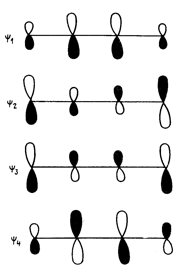
\includegraphics{MO_but}}
\caption{$\pi$-МО бутадиена \cite{dyachkov2011}.}
\label{fig:MOButadien}
\end{figure}

На рис.\ref{fig:MOButadien} схематически изображены МО бутадиена. 
Смена знака молекулярной орбитали при переходе от одного атома к соседнему,отображено в виде смены цвета, которым закрашена орбиталь. 
Если орбиталь не меняет знак, значит между этими атомами орбиталь ведет себя как связывающиая, в противном случае, как разрыхляющая. 
Видно, что $\psi_1$ полностью связывающая, в отличае от остальных, где в некоторых случаях орбитали разрыхляющие. 
Каждая такая смена знака называется узлом МО, чем их больше тем выше энергия орбитали. 
Следую принципу Паули, $\pi$-электроны в невозмбужденном состоянии занимают только $\psi_1$ и $\psi_2$. 

\begin{figure}[h]
	\begin{center}
		\begin{tikzpicture}[scale=0.5,line cap=round,line join=round,>=triangle 45,x=1.0cm,y=1.0cm]
		\clip(-1.414345895704517,-1.407321942552852) rectangle (12.420585932115458,6.986494469490978);
		\draw (-1.0,3.0)-- (1.0,3.0);
		\draw (-1.0091789447787487,2.8036484924023193)-- (0.9908210552212513,2.8036484924023193);
		\draw (1.0,3.0)-- (1.9812607711317565,4.901720162110766);
		\draw (0.9908210552212513,2.8036484924023193)-- (2.0,0.8981921255776499);
		\draw (1.9812607711317565,4.901720162110766)-- (3.9812607711317565,4.901720162110766);
		\draw (2.0,0.8981921255776499)-- (4.0,0.8981921255776499);
		\draw (6.0,3.0)-- (7.999999147707057,2.9981536059343097);
		\draw (5.990821055221251,2.8036484924023193)-- (7.990820202928308,2.8018020983366285);
		\draw (7.999999147707057,2.9981536059343097)-- (9.0,4.5);
		\draw (7.990820202928308,2.8018020983366285)-- (8.999595931182995,1.3000000510223784);
		\draw (9.0,4.5)-- (10.999999147707056,4.498153605934309);
		\draw (8.999595931182995,1.3000000510223784)-- (10.999595078890051,1.2981536569566916);
		\draw (6.0,3.2)-- (8.0,3.2);
		\draw (6.0,2.6)-- (8.0,2.6);
		\draw (7.999999147707057,2.9981536059343097)-- (9.0,6.0);
		\draw (7.990820202928308,2.8018020983366285)-- (9.0,0.0);
		\draw (9.0,6.0)-- (11.0,6.0);
		\draw (9.0,0.0)-- (11.0,0.0);
		\draw (3.043274575341605,2.096892676067388) node[anchor=north west] {$E_1$};
		\draw (3.1248164132265948,6.090067474029987) node[anchor=north west] {$E_2$};
		\draw (10.110233858707407,1.2004656806063962) node[anchor=north west] {$E_1$};
		\draw (10.055872633450747,2.5043594921860204) node[anchor=north west] {$E_2$};
		\draw (10.055872633450747,5.682600657911355) node[anchor=north west] {$E_3$};
		\draw (10.164595083964068,7.1494811959384315) node[anchor=north west] {$E_4$};
		\end{tikzpicture}
		\caption{Первая картинка}
	\end{center}
\end{figure}

\clearpage